\documentclass[11pt]{article}
\usepackage{amsmath,amsbsy,amssymb,verbatim,fullpage,ifthen,graphicx,bm,amsfonts,amsthm,url}
\usepackage{graphicx}
\usepackage{xcolor}
\newcommand{\mfile}[1]  {{\small \verbatiminput{./#1}}} % Jeff Fessler, input matlab file
\newcommand{\tmop}[1]{\ensuremath{\operatorname{#1}}}
%\newcommand*{\qed}{\hfill\ensuremath{\blacksquare}}%
\newcommand{\R}{\mathbb{R}}
\newcommand{\C}{\mathbb{C}}
\newcommand{\Z}{\mathbb{Z}}
\newcommand{\A}{\mathcal{A}}
\newcommand{\minimize}{\operatorname*{minimize\ }}
\newcommand{\maximize}{\operatorname*{maximize}}
\newcommand{\opdet}[1]{\operatorname{\textbf{det}}\left(#1\right)}
\newcommand{\optr}[1]{\operatorname{\textbf{tr}}\left(#1\right)}
%\newcommand{\AnswerDefine}{}
\newcommand{\answer}[2][blue]{\ifdefined\AnswerDefine{\color{#1}\it#2}\fi}
\newcommand{\mtx}[1]{\mathbf{#1}}
\newcommand{\vct}[1]{\mathbf{#1}}
\def \lg       {\langle}
\def \rg       {\rangle}
\def \mA {\mtx{A}}
\def \mF {\mtx{F}}
\def \mG {\mtx{G}}
\def \mI {\mtx{I}}
\def \mJ {\mtx{J}}
\def \mU {\mtx{U}}
\def \mS {\mtx{S}}
\def \mV {\mtx{V}}
\def \mW {\mtx{W}}
\def \mLambda {\mtx{\Lambda}}
\def \mSigma {\mtx{\Sigma}}
\def \mX {\mtx{X}}
\def \mY {\mtx{Y}}
\def \mZ {\mtx{Z}}
\def \zero     {\mathbf{0}}
\def \vzero    {\vct{0}}
\def \vone    {\vct{1}}
\def \va {\vct{a}}
\def \vg {\vct{g}}
\def \vu {\vct{u}}
\def \vv {\vct{v}}
\def \vx {\vct{x}}
\def \vy {\vct{y}}
\def \vz {\vct{z}}
\def \vphi {\vct{\phi}}
\def \vmu {\vct{\mu}}
\def \R {\mathbb{R}}

%\newcommand{\st}{\operatorname*{\ subject\ to\ }}
\usepackage{algorithm,algpseudocode}
\usepackage{xspace}
% Add a period to the end of an abbreviation unless there's one
% already, then \xspace.
\makeatletter
\DeclareRobustCommand\onedot{\futurelet\@let@token\@onedot}
\def\@onedot{\ifx\@let@token.\else.\null\fi\xspace}

\def\eg{\emph{e.g}\onedot} \def\Eg{\emph{E.g}\onedot}
\def\ie{\emph{i.e}\onedot} \def\Ie{\emph{I.e}\onedot}
\def\cf{\emph{c.f}\onedot} \def\Cf{\emph{C.f}\onedot}
\def\etc{\emph{etc}\onedot} \def\vs{\emph{vs}\onedot}
\def\wrt{w.r.t\onedot} \def\dof{d.o.f\onedot}
\def\etal{\emph{et al}\onedot} \def\st{\emph{s.t}\onedot}
\pagestyle{plain}

\title{{\bf Homework Set 3, CPSC 8420, Spring 2022}} % Change to the appropriate homework number
\author{\Large\underline{Song, Zhiyuan}}
\date{\today} % put your name in the LastName, FirstName format

\begin{document}
\maketitle

\section*{Problem 1}
Data points were centered when they were dealt with PCA and LDA. Thep projection lines crossed the center of the points. If centered data points were scatter-plotted, the projection lines should have crossed the origin.
\begin{figure}
	\centering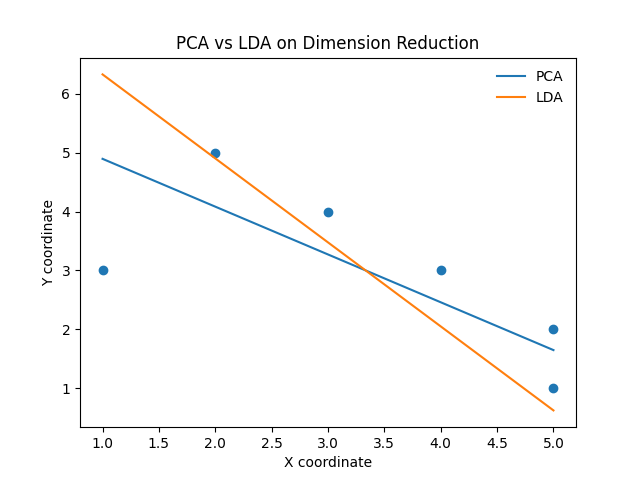
\includegraphics[width=.75\linewidth]{prob1.png}
	\caption{\textbf{Dimension Reduction using PCA and LDA} } % caption of the figure
	\label{fig:p1}
\end{figure}
\mfile{prob1.py}
\section*{Problem 2}
Given positive data-set $\{\{1,1\},\{2,2\},\{2,3\}\}$, as well as negative data-set $\{\{3,2\},\{3,3\},\{4,4\}\}$, please determine the decision boundary when leveraging $k$-NN where $k=1$ and $k=3$ respectively.\\
Boundaries were determined using different $k$.
\mfile{prob2.py}
\begin{figure}
	\centering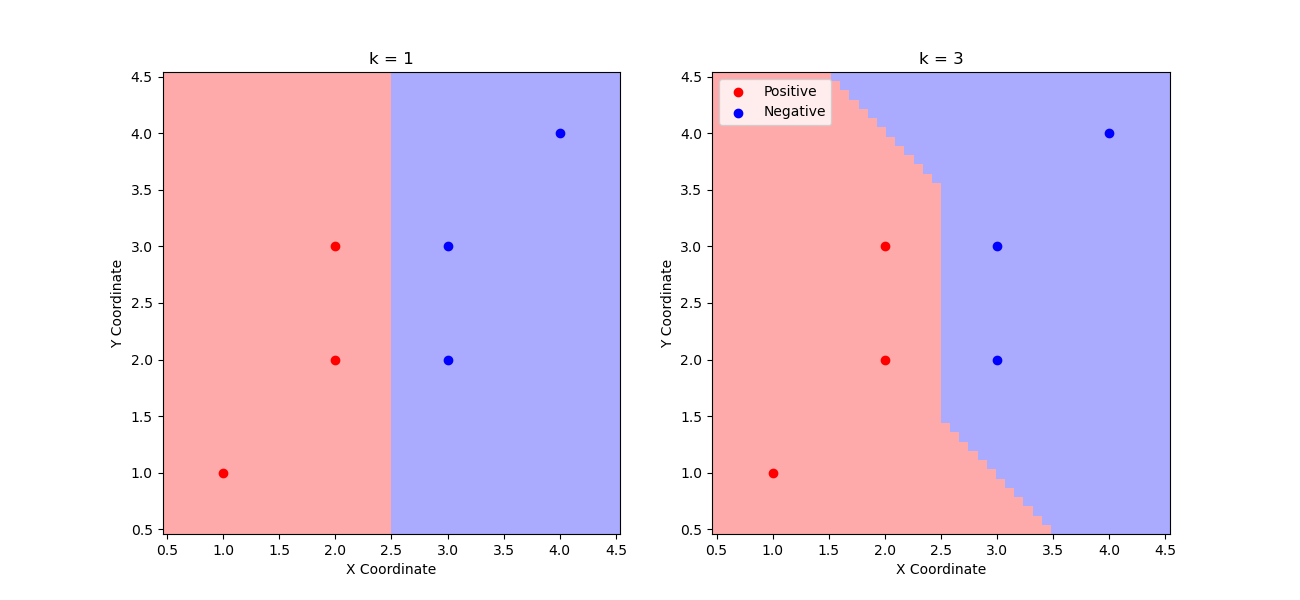
\includegraphics[width=1\linewidth]{prob2.png}
	\caption{\textbf{$K-NN$ Bundary Determination with Different $k$} } % caption of the figure
	\label{fig:p2}
\end{figure}

\section*{Problem 3}
Given SPD matrices $X, Y, Z$, now please follow the idea/method used in LDA/PCA to find the best solution to:
\begin{equation}\label{eq1}
\begin{aligned}
&\underbrace{arg\;max}_{a,b}\;\;{a^TZb}\\
s.t. \ \ &a^TXa =1,\; b^TYb =1
\end{aligned}
\end{equation}
Applying Lagrange multiplier to this optimization problem, Eq.\ref{eq1} is equivalent to
\begin{align}\label{eq2}
&\min_{a,b,\lambda,\beta}\;\;{-a^TZb+\frac{1}{2}\lambda\left(a^TXa-1\right)+\frac{1}{2}\beta\left(b^TYb-1\right)}
\end{align}
Let $f=-a^TZb+\lambda\left(a^TXa-1\right)+\beta\left(b^TYb-1\right)$, we can get condition-constrained equations by taking partial derivative and make differential eqatuions equal to zero, respected to $a,b,\lambda,\beta$, respectively.
\begin{align}\label{eq3}
\frac{\partial f}{\partial a}=-Zb+\lambda S_Xa=-Zb+\lambda Xa=0
\end{align}
\begin{align}\label{eq4}
\frac{\partial f}{\partial b}=-Z^Ta+\beta S_Yb=-Z^Ta+\beta Yb=0
\end{align}
Where $S_X$ and $S_Y$ are the symmetric part of the X and Y, respectively. In general, $S_A=\frac{1}{2}\left(A+A^T\right)$. In the case of a SPD matrix $A$,$S_A=A$. Besides, other two derivatives will lead to constrains, as shown below.
\begin{align*}
\frac{\partial f}{\partial \lambda}=a^TXa-1=0\\
\frac{\partial f}{\partial \beta}=b^TYb-1=0
\end{align*}
If we manipulate Eq.\ref{eq3} with left multiply $a^T$, we will get $a^TZb=\lambda a^TXa=\lambda$. Similarly, we can also obtain $b^TZa=\beta$ from Eq.\ref{eq4}. Therefore, $\lambda$ and $\beta$ are equivalent. In order to get $\max a^TZb$, we need to maximize either $\lambda$ or $\beta$ ($\lambda$ used in the later context).
We can obtain the expression of $b$ in terms of $a$ using Eq.\ref{eq3}, $b=\lambda Z^{-1}Xa$, and plug it into Eq.\ref{eq4}. Consequently, we can get
\begin{align*}
Za=\lambda\beta YZ^{-1}Xa
\end{align*}
\begin{align}\label{eq5}
X^{-1}ZY^{-1}Za=\lambda^2a
\end{align}
Similarly, we can express $a$ in terms of $b$ from Eq.\ref{eq4} and plug it into Eq.\ref{eq4} to get the equation for b.
\begin{align}\label{eq6}
Y^{-1}ZX^{-1}Zb=\lambda^2b
\end{align}
Eq.\ref{eq5} and \ref{eq6} are nothing but eigenvalue problems for matrices $\mtx{A}=X^{-1}ZY^{-1}Z$ and $\mtx{B}=Y^{-1}ZX^{-1}Z$, respectively.\\
Besides, we can notice that matrices $\mA$ and $\mtx{B}$ can be expressed as
\begin{align*}
\mA=\mU\mtx{M}\\
\mtx{B}=\mtx{M}\mU
\end{align*}
where $\mU=X^{-1}Z$ and $\mtx{M}=Y^{-1}Z$. In the eigenvalues decomposition on $A$ and $B$, we know that $UM$ and $MU$ have the same eigenvalues. Therefore, Eq.\ref{eq5} and Eq.\ref{eq6} can result in the same eigenvalues for $\lambda^2$ from $[W_A,V_A]=\text{eig}(A)$ and $[W_B,V_B]=\text{eig}(B)$. Meanwhile, matrices $X$, $Y$ and $Z$ are all SPD, leading to the eigenvalues for either $A$ or $B$ are non-negative real numbers. We can simply sort the eigenvalues and select the eigenvectors corresponding to largest eigenvalue for $a$ and $b$ from $W_A$ amd $W_B$, respectively. As a result, $a^TZb$ can be maximized with the constrains $a^TXa=1$ and $b^TYb=1$.
\end{document}
